\section{CVector$<$ T $>$ Class Template Reference}
\label{classCVector}\index{CVector@{CVector}}
This is a c-style implementation of std::vector.  


{\tt \#include $<$cvector.h$>$}

Inheritance diagram for CVector$<$ T $>$::\begin{figure}[H]
\begin{center}
\leavevmode
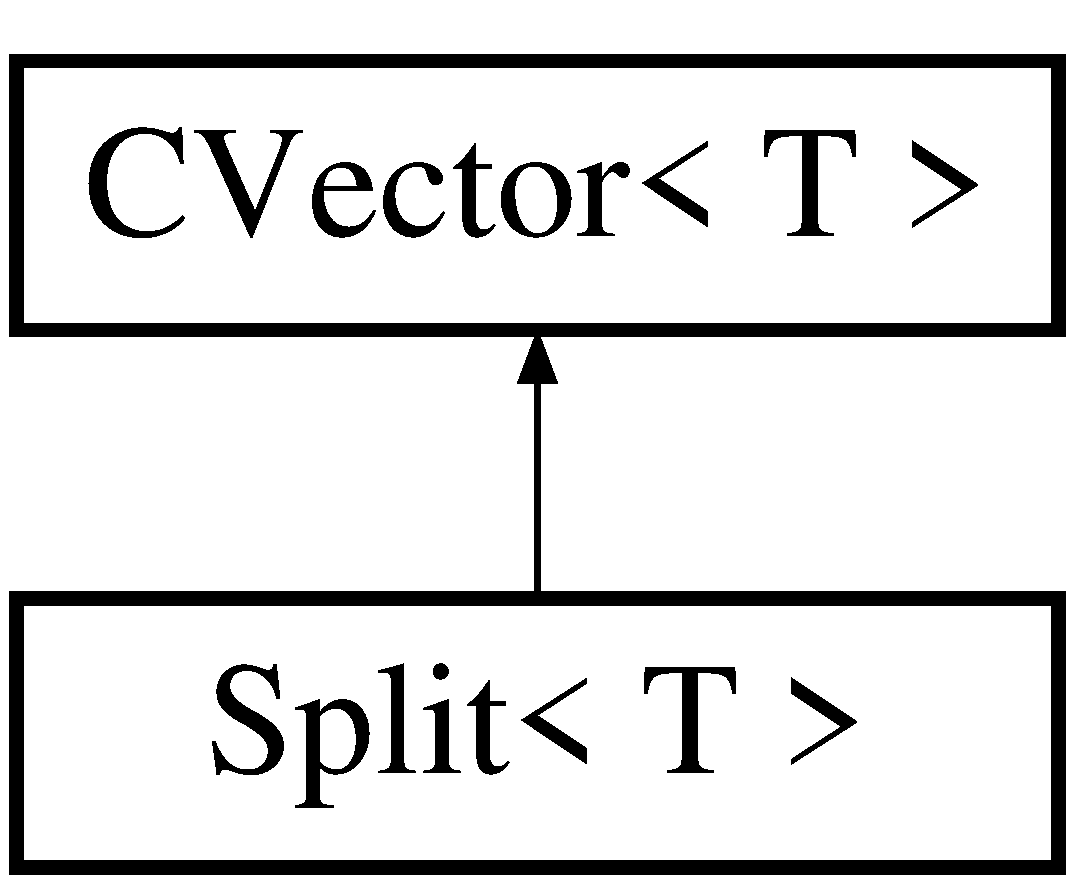
\includegraphics[height=2cm]{classCVector}
\end{center}
\end{figure}
\subsection*{Public Member Functions}
\begin{CompactItemize}
\item 
{\bf CVector} ()
\item 
{\bf CVector} (const {\bf CVector} \&)
\item 
{\bf CVector} (size\_\-t)
\item 
{\bf $\sim$CVector} ()
\item 
{\bf CVector} \& {\bf operator=} (const {\bf CVector} \&)
\item 
T \& {\bf operator[$\,$]} (size\_\-t)
\item 
T \& {\bf at} (size\_\-t)
\item 
const T \& {\bf operator[$\,$]} (size\_\-t) const 
\item 
const T \& {\bf at} (size\_\-t) const 
\item 
void {\bf push\_\-back} (const T \&)
\item 
void {\bf pop\_\-back} ()
\item 
void {\bf reserve} (size\_\-t)
\item 
void {\bf clear} ()
\item 
size\_\-t {\bf size} () const 
\item 
void {\bf set\-Size} (size\_\-t)
\item 
bool {\bf empty} () const 
\end{CompactItemize}
\subsection*{Static Public Attributes}
\begin{CompactItemize}
\item 
static double {\bf \_\-growth\-Factor} = 1.5
\begin{CompactList}\small\item\em Factor to use when resizing: \_\-size = \_\-growth\-Factor $\ast$ \_\-size. \item\end{CompactList}\end{CompactItemize}
\subsection*{Protected Member Functions}
\begin{CompactItemize}
\item 
void {\bf grow} ()
\end{CompactItemize}
\subsection*{Protected Attributes}
\begin{CompactItemize}
\item 
T $\ast$ {\bf \_\-array}
\item 
size\_\-t {\bf \_\-size}
\begin{CompactList}\small\item\em The actual memory block. \item\end{CompactList}\item 
size\_\-t {\bf \_\-cap}
\begin{CompactList}\small\item\em The number of elements. \item\end{CompactList}\end{CompactItemize}


\subsection{Detailed Description}
\subsubsection*{template$<$class T$>$ class CVector$<$ T $>$}

This is a c-style implementation of std::vector. 

It is designed for PODs (plain old datatypes) ie objects without constructors and uses realloc() to request new memory. The assumption is realloc() is potentially more efficient than new() as it can sometimes increase the reserved memory without having to copy the current contents. 



\subsection{Constructor \& Destructor Documentation}
\index{CVector@{CVector}!CVector@{CVector}}
\index{CVector@{CVector}!CVector@{CVector}}
\subsubsection{\setlength{\rightskip}{0pt plus 5cm}template$<$class T$>$ {\bf CVector}$<$ T $>$::{\bf CVector} ()\hspace{0.3cm}{\tt  [inline]}}\label{classCVector_a0}


\index{CVector@{CVector}!CVector@{CVector}}
\index{CVector@{CVector}!CVector@{CVector}}
\subsubsection{\setlength{\rightskip}{0pt plus 5cm}template$<$class T$>$ {\bf CVector}$<$ T $>$::{\bf CVector} (const {\bf CVector}$<$ T $>$ \&)\hspace{0.3cm}{\tt  [inline]}}\label{classCVector_a1}


\index{CVector@{CVector}!CVector@{CVector}}
\index{CVector@{CVector}!CVector@{CVector}}
\subsubsection{\setlength{\rightskip}{0pt plus 5cm}template$<$class T$>$ {\bf CVector}$<$ T $>$::{\bf CVector} (size\_\-t)\hspace{0.3cm}{\tt  [inline]}}\label{classCVector_a2}


\index{CVector@{CVector}!~CVector@{$\sim$CVector}}
\index{~CVector@{$\sim$CVector}!CVector@{CVector}}
\subsubsection{\setlength{\rightskip}{0pt plus 5cm}template$<$class T$>$ {\bf CVector}$<$ T $>$::$\sim${\bf CVector} ()\hspace{0.3cm}{\tt  [inline]}}\label{classCVector_a3}




\subsection{Member Function Documentation}
\index{CVector@{CVector}!at@{at}}
\index{at@{at}!CVector@{CVector}}
\subsubsection{\setlength{\rightskip}{0pt plus 5cm}template$<$class T$>$ const T \& {\bf CVector}$<$ T $>$::at (size\_\-t) const\hspace{0.3cm}{\tt  [inline]}}\label{classCVector_a8}


\index{CVector@{CVector}!at@{at}}
\index{at@{at}!CVector@{CVector}}
\subsubsection{\setlength{\rightskip}{0pt plus 5cm}template$<$class T$>$ T \& {\bf CVector}$<$ T $>$::at (size\_\-t)\hspace{0.3cm}{\tt  [inline]}}\label{classCVector_a6}


\index{CVector@{CVector}!clear@{clear}}
\index{clear@{clear}!CVector@{CVector}}
\subsubsection{\setlength{\rightskip}{0pt plus 5cm}template$<$class T$>$ void {\bf CVector}$<$ T $>$::clear ()\hspace{0.3cm}{\tt  [inline]}}\label{classCVector_a12}


\index{CVector@{CVector}!empty@{empty}}
\index{empty@{empty}!CVector@{CVector}}
\subsubsection{\setlength{\rightskip}{0pt plus 5cm}template$<$class T$>$ bool {\bf CVector}$<$ T $>$::empty () const\hspace{0.3cm}{\tt  [inline]}}\label{classCVector_a15}


\index{CVector@{CVector}!grow@{grow}}
\index{grow@{grow}!CVector@{CVector}}
\subsubsection{\setlength{\rightskip}{0pt plus 5cm}template$<$class T$>$ void {\bf CVector}$<$ T $>$::grow ()\hspace{0.3cm}{\tt  [protected]}}\label{classCVector_b0}


\index{CVector@{CVector}!operator=@{operator=}}
\index{operator=@{operator=}!CVector@{CVector}}
\subsubsection{\setlength{\rightskip}{0pt plus 5cm}template$<$class T$>$ {\bf CVector}$<$ T $>$ \& {\bf CVector}$<$ T $>$::operator= (const {\bf CVector}$<$ T $>$ \&)\hspace{0.3cm}{\tt  [inline]}}\label{classCVector_a4}


\index{CVector@{CVector}!operator[]@{operator[]}}
\index{operator[]@{operator[]}!CVector@{CVector}}
\subsubsection{\setlength{\rightskip}{0pt plus 5cm}template$<$class T$>$ const T \& {\bf CVector}$<$ T $>$::operator[$\,$] (size\_\-t) const\hspace{0.3cm}{\tt  [inline]}}\label{classCVector_a7}


\index{CVector@{CVector}!operator[]@{operator[]}}
\index{operator[]@{operator[]}!CVector@{CVector}}
\subsubsection{\setlength{\rightskip}{0pt plus 5cm}template$<$class T$>$ T \& {\bf CVector}$<$ T $>$::operator[$\,$] (size\_\-t)\hspace{0.3cm}{\tt  [inline]}}\label{classCVector_a5}


\index{CVector@{CVector}!pop_back@{pop\_\-back}}
\index{pop_back@{pop\_\-back}!CVector@{CVector}}
\subsubsection{\setlength{\rightskip}{0pt plus 5cm}template$<$class T$>$ void {\bf CVector}$<$ T $>$::pop\_\-back ()\hspace{0.3cm}{\tt  [inline]}}\label{classCVector_a10}


\index{CVector@{CVector}!push_back@{push\_\-back}}
\index{push_back@{push\_\-back}!CVector@{CVector}}
\subsubsection{\setlength{\rightskip}{0pt plus 5cm}template$<$class T$>$ void {\bf CVector}$<$ T $>$::push\_\-back (const T \&)\hspace{0.3cm}{\tt  [inline]}}\label{classCVector_a9}


\index{CVector@{CVector}!reserve@{reserve}}
\index{reserve@{reserve}!CVector@{CVector}}
\subsubsection{\setlength{\rightskip}{0pt plus 5cm}template$<$class T$>$ void {\bf CVector}$<$ T $>$::reserve (size\_\-t)\hspace{0.3cm}{\tt  [inline]}}\label{classCVector_a11}


\index{CVector@{CVector}!setSize@{setSize}}
\index{setSize@{setSize}!CVector@{CVector}}
\subsubsection{\setlength{\rightskip}{0pt plus 5cm}template$<$class T$>$ void {\bf CVector}$<$ T $>$::set\-Size (size\_\-t)\hspace{0.3cm}{\tt  [inline]}}\label{classCVector_a14}


\index{CVector@{CVector}!size@{size}}
\index{size@{size}!CVector@{CVector}}
\subsubsection{\setlength{\rightskip}{0pt plus 5cm}template$<$class T$>$ size\_\-t {\bf CVector}$<$ T $>$::size () const\hspace{0.3cm}{\tt  [inline]}}\label{classCVector_a13}




\subsection{Member Data Documentation}
\index{CVector@{CVector}!_array@{\_\-array}}
\index{_array@{\_\-array}!CVector@{CVector}}
\subsubsection{\setlength{\rightskip}{0pt plus 5cm}template$<$class T$>$ T$\ast$ {\bf CVector}$<$ T $>$::{\bf \_\-array}\hspace{0.3cm}{\tt  [protected]}}\label{classCVector_p0}


\index{CVector@{CVector}!_cap@{\_\-cap}}
\index{_cap@{\_\-cap}!CVector@{CVector}}
\subsubsection{\setlength{\rightskip}{0pt plus 5cm}template$<$class T$>$ size\_\-t {\bf CVector}$<$ T $>$::{\bf \_\-cap}\hspace{0.3cm}{\tt  [protected]}}\label{classCVector_p2}


The number of elements. 

\index{CVector@{CVector}!_growthFactor@{\_\-growthFactor}}
\index{_growthFactor@{\_\-growthFactor}!CVector@{CVector}}
\subsubsection{\setlength{\rightskip}{0pt plus 5cm}template$<$class T$>$ double {\bf CVector}$<$ T $>$::{\bf \_\-growth\-Factor} = 1.5\hspace{0.3cm}{\tt  [static]}}\label{classCVector_s0}


Factor to use when resizing: \_\-size = \_\-growth\-Factor $\ast$ \_\-size. 

\index{CVector@{CVector}!_size@{\_\-size}}
\index{_size@{\_\-size}!CVector@{CVector}}
\subsubsection{\setlength{\rightskip}{0pt plus 5cm}template$<$class T$>$ size\_\-t {\bf CVector}$<$ T $>$::{\bf \_\-size}\hspace{0.3cm}{\tt  [protected]}}\label{classCVector_p1}


The actual memory block. 



The documentation for this class was generated from the following files:\begin{CompactItemize}
\item 
{\bf cvector.h}\item 
{\bf cvector\_\-impl.h}\end{CompactItemize}
